\chapter{IMPLEMENTATION AND TESTING}


% (20\% of Report Length)

% a. Showcase the output at various intermediate stages of the project pipeline

% b. Use proper data visualizing techniques to present the output

% c. Figures and tables must be accompanied by an explanation
\section{System Development Tools}\textbf{HTML:}\\
HTML, or Hypertext Markup Language, constitutes the backbone of web development by providing the structural foundation for web content. Utilizing a system of tags, HTML defines the arrangement of content elements on a webpage. These tags encapsulate diverse elements, such as headings, paragraphs, images, links, and forms, which compose the web interface. HTML's hierarchical structure reflects the logical flow of information, enhancing accessibility and readability for both users and developers.\\\\
\textbf{PHP:}\\
PHP, or Hypertext Preprocessor, empowers web apps with server-side capabilities for data manipulation, database interaction, and dynamic content generation. It handles form inputs, manages user sessions, and enforces authentication. PHP also performs server-side validation, data processing, and complex backend logic, making it ideal for enhancing platforms like PC part pickers. It seamlessly integrates with JavaScript via AJAX, enabling real-time updates without page reloads, ensuring users receive accurate information and a smooth, interactive experience.\\\\
\textbf{JavaScript:}\\
JavaScript is a versatile scripting language that enables interactivity and dynamic behavior on web pages. It runs directly in the browser, allowing developers to create responsive and engaging user experiences. JavaScript adds a layer of functionality that HTML and CSS alone cannot achieve, making it an essential tool in modern web development.\\\\
\textbf{Figma:}\\
Figma is a cloud-based design tool that plays a vital role in the initial design and prototyping phases of web development. It fosters collaboration among designers and developers, streamlines the design process, and ensures a cohesive and user-centered visual design for the platform.\\\\
\newpage
\textbf{Bootstrap:}\\
Bootstrap is a popular, open-source front-end web framework for designing responsive and mobile-first web pages and applications. It was originally developed by Twitter, and it is now maintained by volunteers through GitHub. Bootstrap provides pre-built design components, CSS (Cascading Style Sheets) frameworks, and JavaScript plugins, making it easier and faster to create consistent, visually appealing, and functional web interfaces.\\\\
\textbf{JQuery:}\\
jQuery is a widely-used JavaScript library that simplifies web development. It provides a collection of pre-built functions and plugins for interacting with HTML documents, handling events, and making asynchronous requests. jQuery streamlines client-side scripting, making it easier to create interactive and dynamic web pages. Its concise syntax and cross-browser compatibility have made it a popular choice for developers seeking to enhance user interfaces and improve the overall user experience on websites and web applications.
% \subsection{Implementation Details of Modules}
\newpage
 \section{Testing}
 \subsection{Test Cases for Unit Testing}
Unit testing is a software testing technique where individual units or components of a software application are tested in isolation to ensure that they function correctly. These units can be functions, methods, classes, or even small modules. Unit testing aims to verify that each unit performs as expected, providing developers with confidence that their code works as intended and catches bugs early in the development process.
\\
\begin{figure}[H]
    \end{figure}
    \begin{table}[H]
        \caption{Unit Test Cases of home/index.php in Build Wizard}
            \label{}
            \begin{tabularx}{\textwidth}{|>{\raggedright\arraybackslash}p{0.3in}|X|>{\raggedright\arraybackslash}p{2in}|X|X|}
                \hline
                Tests & Scenario & Expected Output & Actual Output \\
                \hline
                    1 & GETmethod: favourites =true & User Portal with favourite item & favourite list with description \\
                    \hline
                    2 & GETmethod: search= intel & Shows components of intel & Shows components of intel \\
                    \hline
                    3 & POSTmethod: estimate & Shows estimates of build & shows estimated price\\
                    \hline
    \end{tabularx}
    \end{table}
\newpage
\subsection{Test Cases for System Testing}
Here testing different test cases of authentication system in BuildWizard : Pcpart picker is performed with screenshots as required results:\\
\begin{table}[H]
    \caption{Authentication Test Cases}
        \label{}
        \begin{tabularx}{\textwidth}{|>{\raggedright\arraybackslash}p{0.3in}|X|>{\raggedright\arraybackslash}p{2in}|X|X|}
            \hline
            Tests & Test Cases & Input & Output \\
            \hline
                1 & signup& Email:sirjan2@gmail.com Password:sirjan1234& signup \\
                \hline
                2 & Incorrect  Password in SignIn & Email:sirjan2@gmail.com
                Password:12345679
                Password:12345678 & Password Incorrect \\
                \hline
                3 & Correct Credentials In Login & Email:sirjan2@gmail.com
                Password:sirjan1234 & Redirects to homepage \\
                \hline
\end{tabularx}
\end{table}
 In given below figure we are testing sigin and signup with incorrect and correct authentication.

    \begin{figure}[H]
    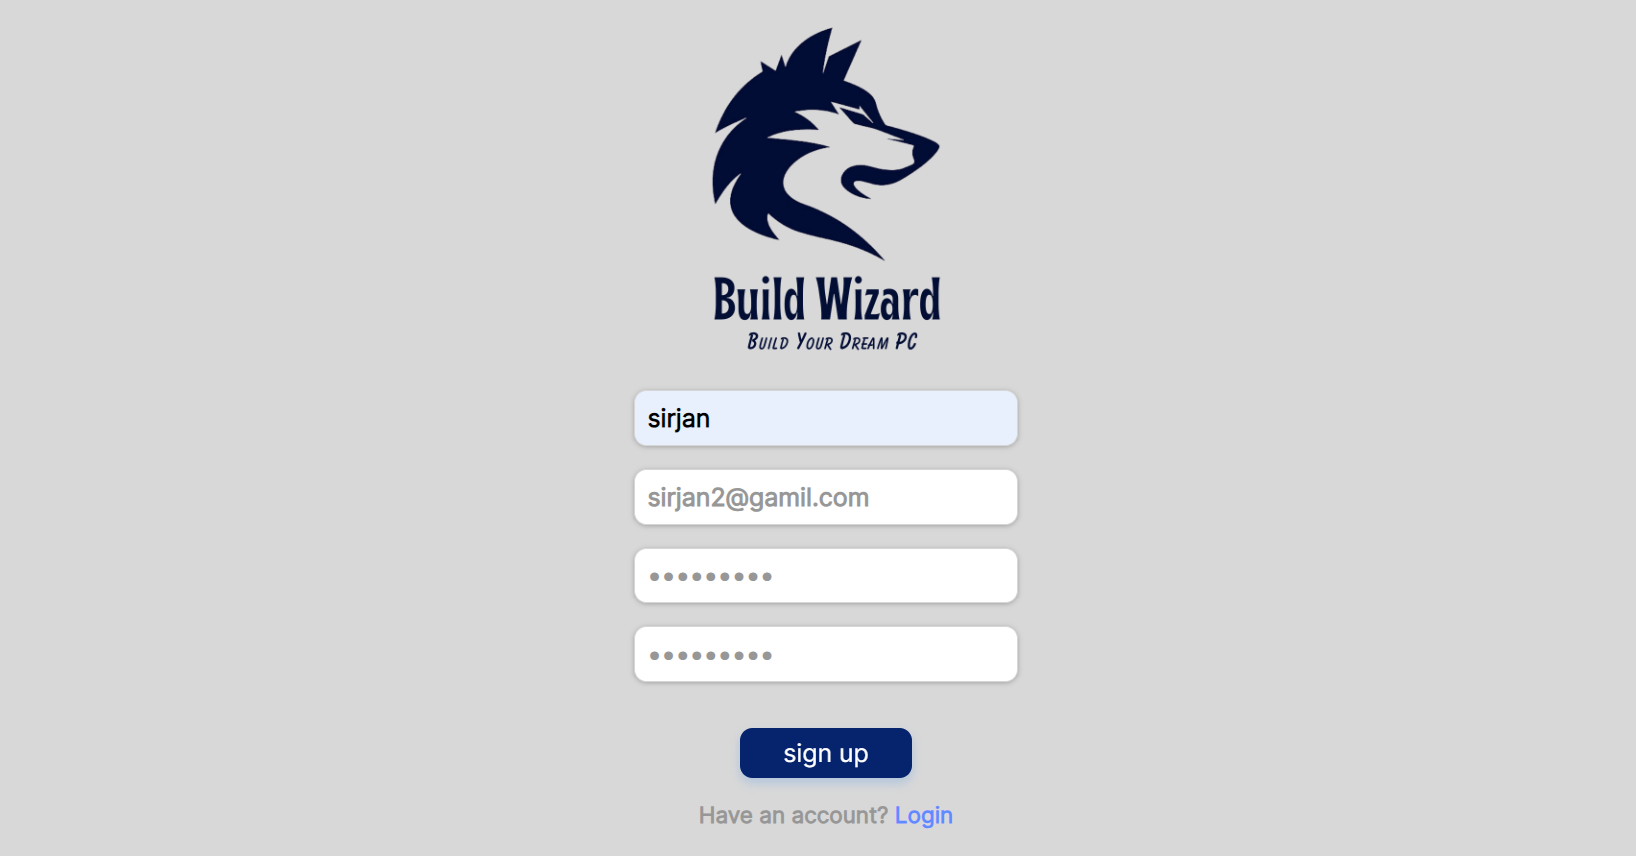
\includegraphics[width=15cm]{Diagrams/sucesssignup.png}
    \caption{Sucessfull SignUp}
    \end{figure}
    \begin{table}[H]
        \caption{Launch Application}
            \label{}
            \begin{tabularx}{\textwidth}{|>{\raggedright\arraybackslash}p{0.3in}|X|>{\raggedright\arraybackslash}p{2in}|X|X|}
                \hline
                Tests & Test Cases & Input & Expected Output & Actual Output \\
                \hline
                    1 & Launch Application & \url{http://localhost/pbw/home/}& Home page & Home page \\
                    \hline
    \end{tabularx}
    \end{table}
    \begin{figure}[H]
    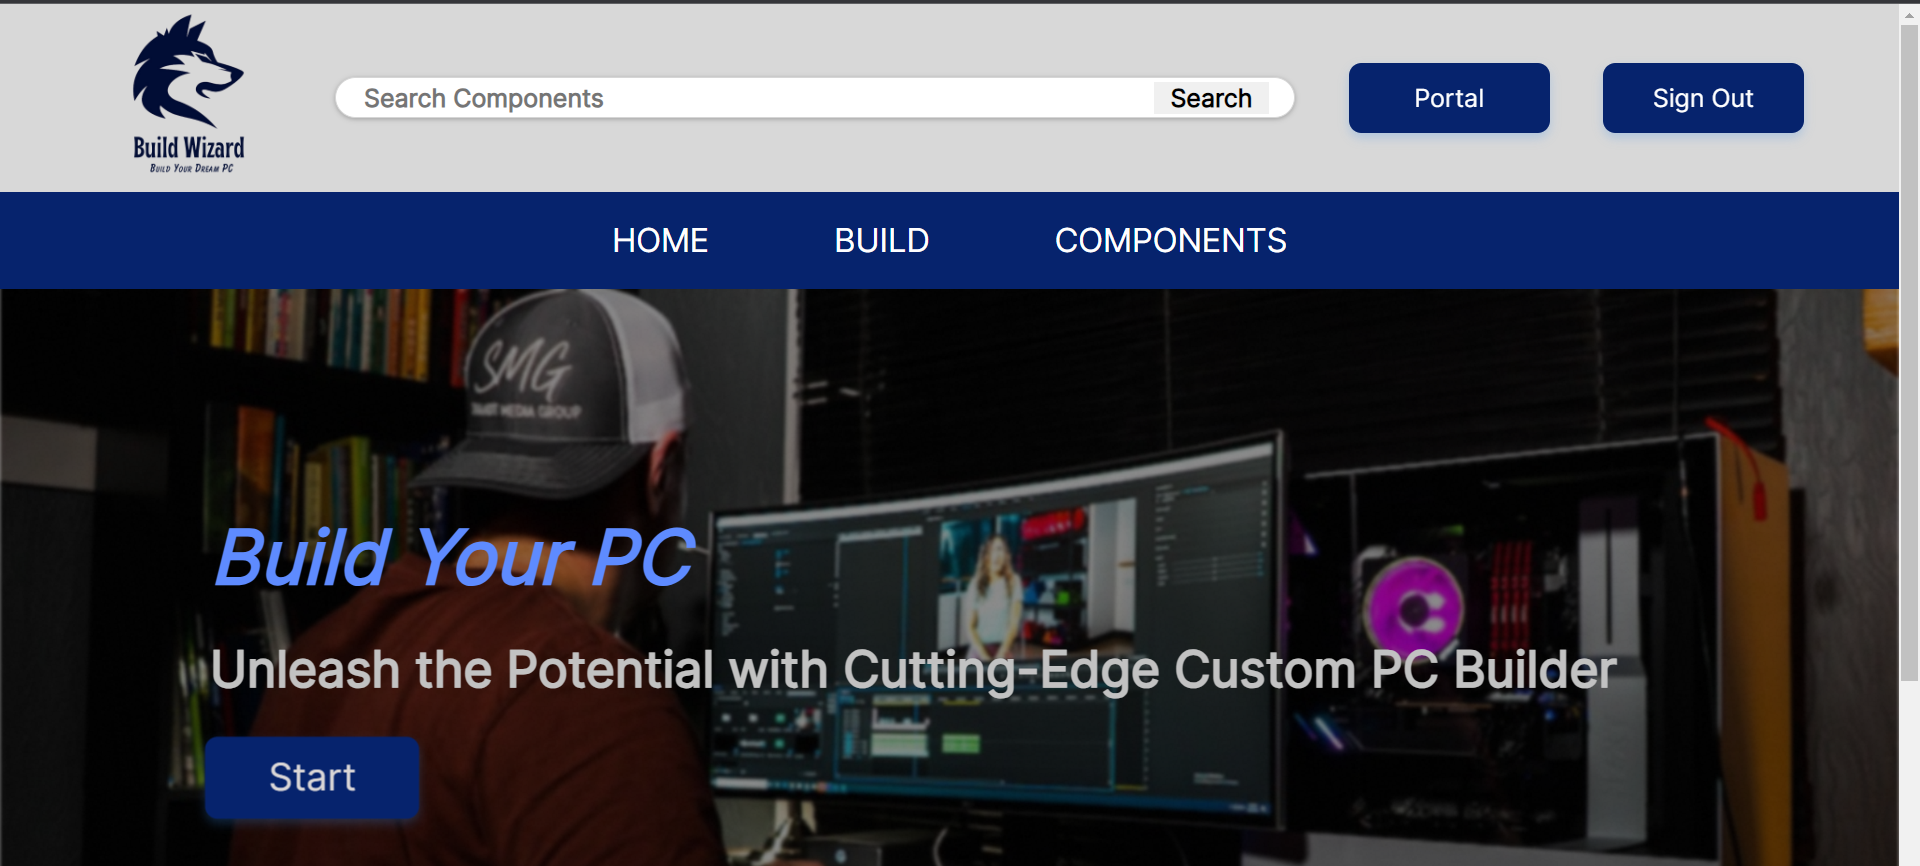
\includegraphics[width=15cm]{Diagrams/sucessloginpage.png}
    \caption{Successful Login}
    \end{figure}
    % admin portal}
    \newpage
        \begin{table}[H]
            \caption{Add component by Admin}
                \label{}
                \begin{tabularx}{\textwidth}{|>{\raggedright\arraybackslash}p{0.3in}|X|>{\raggedright\arraybackslash}p{2in}|X|X|}
                    \hline
                    Tests & Test Cases & Input & Expected Output & Actual Output \\
                    \hline
                        1 & Add components/Manage CPU  & \url{http://localhost/pbw/adminportal/?manage=cpu} & Add product details in form  & opens cpu form  \\
                        \hline
                        2 & Delete components/Manage CPU & \url{http://localhost/pbw/adminportal/?manage=cpu}
                        & Manage Product list & Remove unwanted components\\
                        \hline
        \end{tabularx}
        \end{table}
        \begin{figure}[H]
            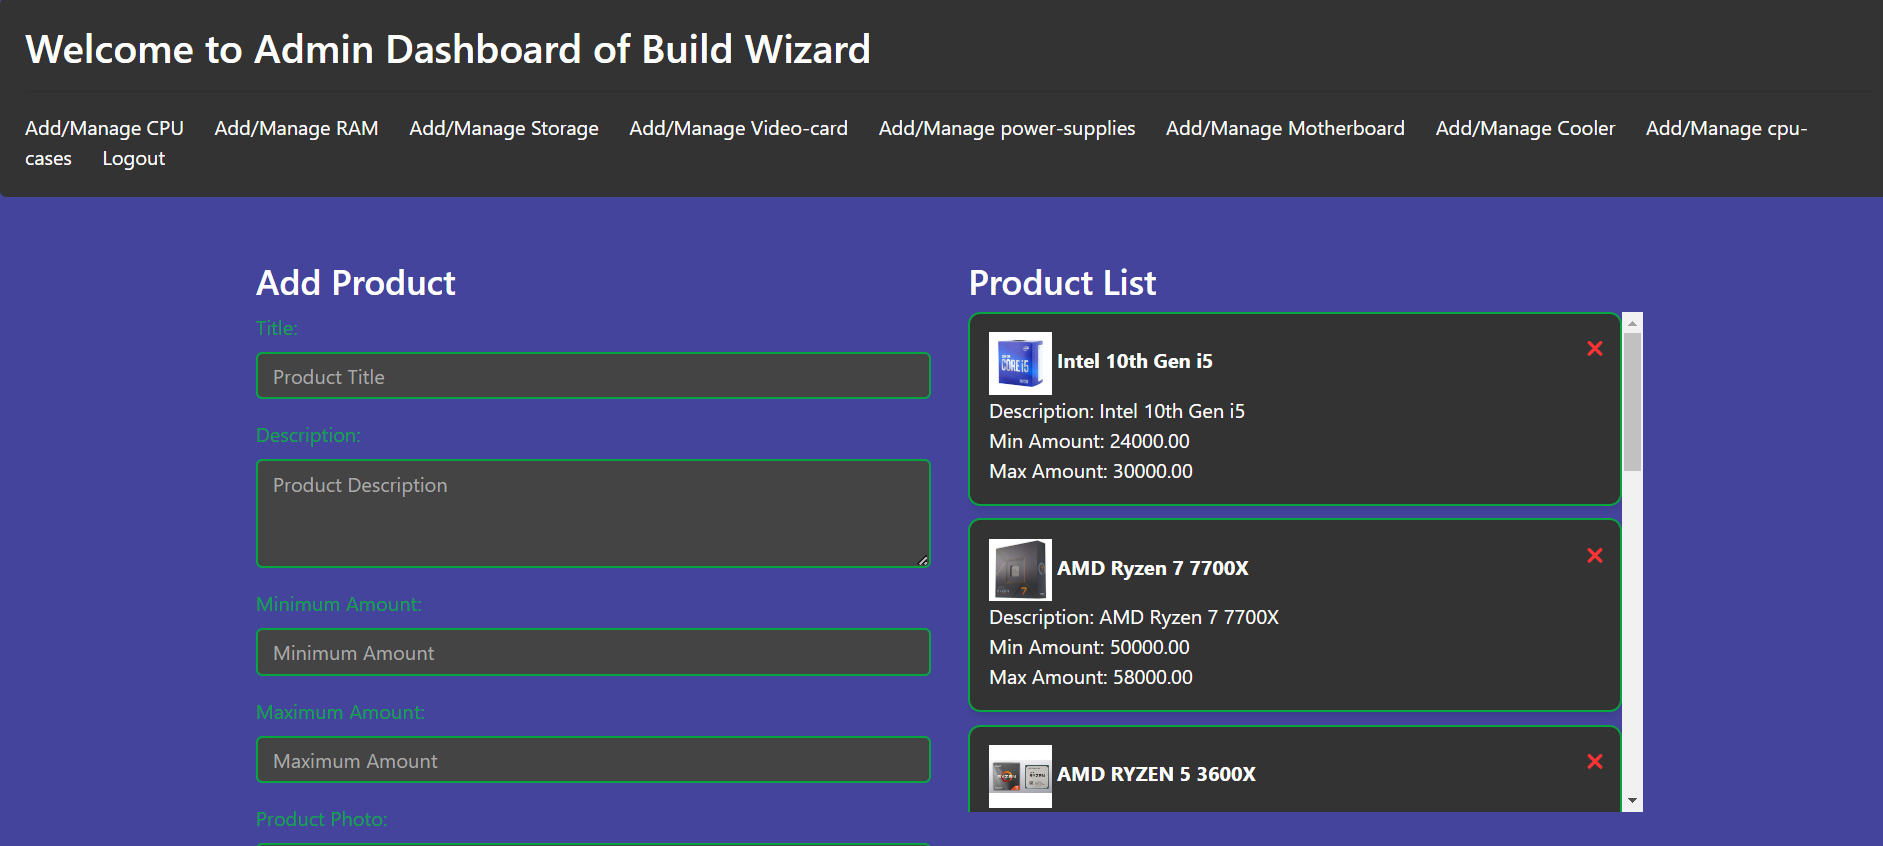
\includegraphics[width=15cm]{Diagrams/admin_portal.png}
            \caption{Add component by Admin}
            \end{figure}
        % components
        \newpage
            \begin{table}[H]
                \caption{Component page}
                    \label{}
                    \begin{tabularx}{\textwidth}{|>{\raggedright\arraybackslash}p{0.3in}|X|>{\raggedright\arraybackslash}p{2in}|X|X|}
                        \hline
                        Tests & Test Cases & Input & Expected Output & Actual Output \\
                        \hline
                            1 & Show components & \url{http://localhost/pbw/components/} & Components & Shows components  \\
                            \hline
                           2 & Component: RAM  &\url{http://localhost/pbw/products/?component=ram}& shows list of ram& ram details \\
                           \hline
            \end{tabularx}
            \end{table}
            \begin{figure}[H]
                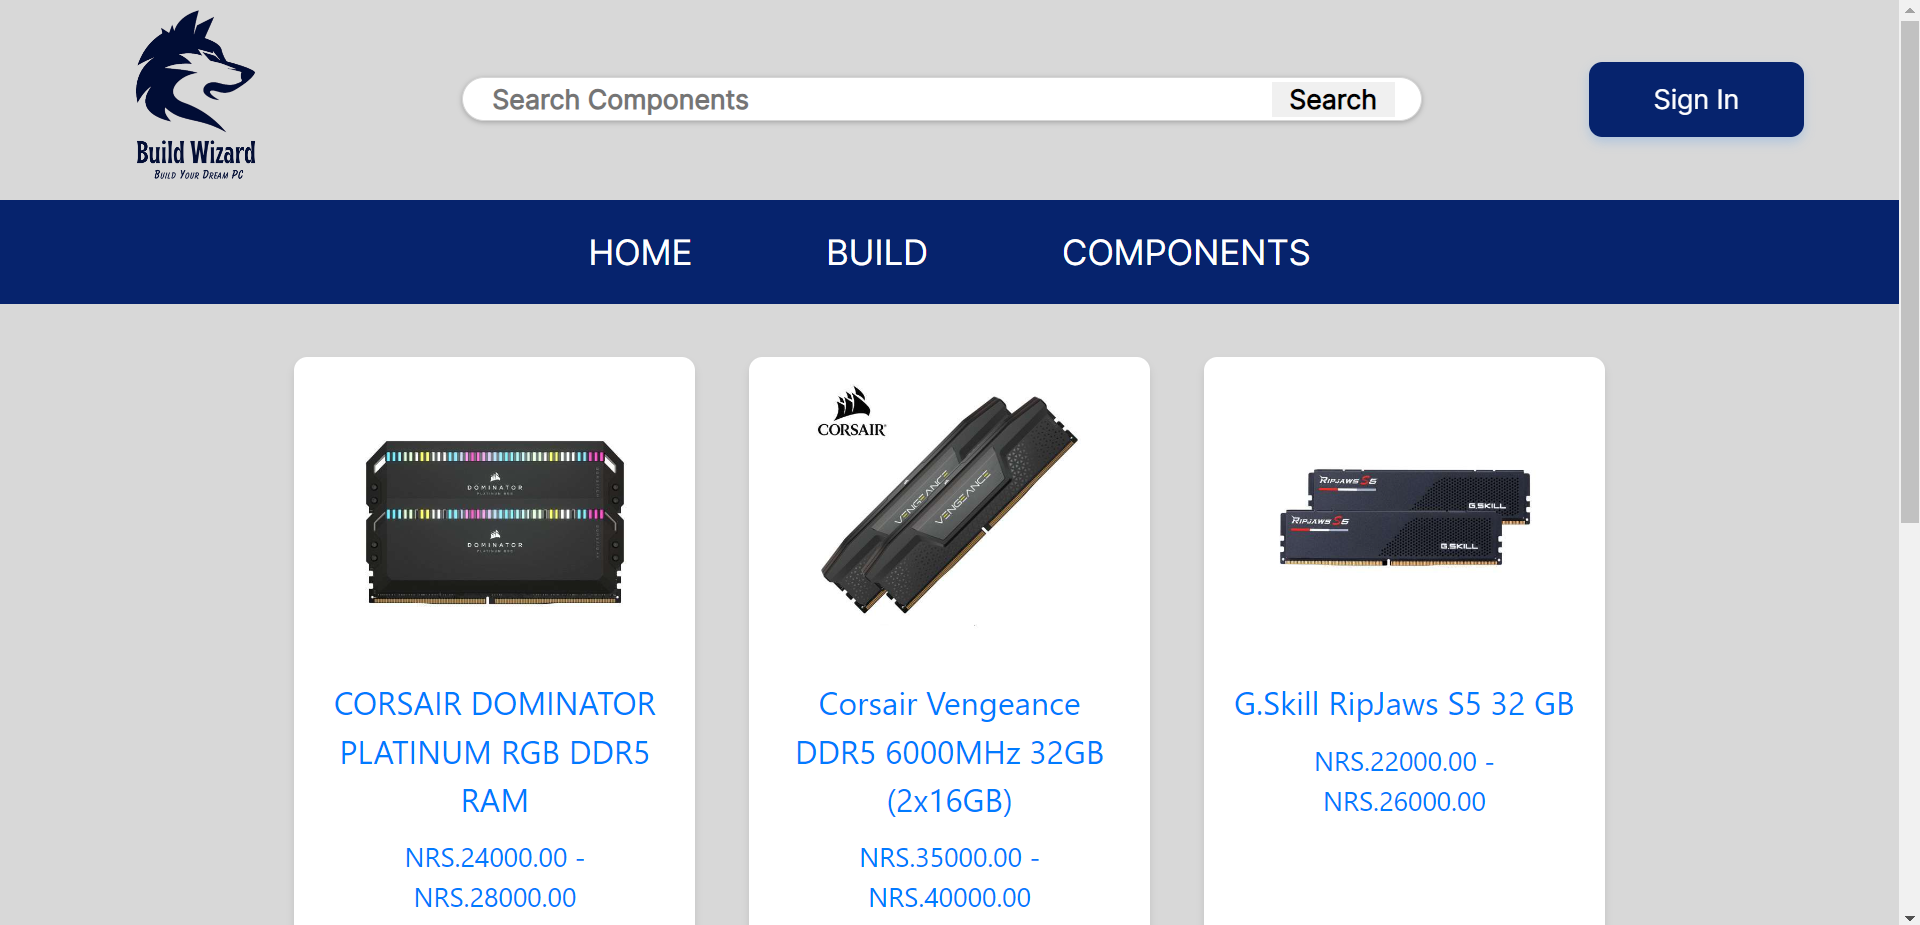
\includegraphics[width=15cm]{Diagrams/rams.png}
                \caption{Components}
                \end{figure}
        

% \subsection{Test Cases for Unit Testing}
% \subsection{Test Cases for System Testing}